\section{Non-idealities (R5)}\label{sec:nonideal}

\subsection{Finite zero depth}
Experimental donuts have a residual intensity $\epsilon$ at the zero, relative to the ring
maximum (below $0.2\%$ in Ref.~\cite{Balzarotti2017}\src{lit_balzarotti_zero_depth}). We model it
in two ways (App.~\ref{app:derivation}): a \emph{constant} pedestal, $I=I_{\mathrm{LG}}+\epsilon$,
and a \emph{Gaussian} pedestal, $I=(ea\rho^2+\epsilon)e^{-a\rho^2}$. The constant pedestal is
exactly a background: at the centre the CRB is Eq.~\eqref{eq:s31} with
$\sbr_\epsilon=3e\,x\,e^{-x}/(4\epsilon)$; the Gaussian pedestal is not equivalent to any
background, because it differs between exposures and reduces the slope of the donut\src{deriv_pedestal}. With $\epsilon>0$ the point value equals the limit and tends, as
$\epsilon\to0$, to the point value $\sigma_{\mathrm{pt}}$, not to $\sigma_{\lim}$.

\emph{Degradation at fixed $L$.} Table~\ref{tab:eps} lists
$\crb(\epsilon)/\sigma_{\mathrm{pt}}$ at the centre. The loss is largest for small $L$, since
$\sbr_\epsilon\propto x\propto L^2$: at $L=50$\,nm a pedestal of $5\%$ roughly doubles the CRB.
The two pedestal models agree to first order in $\epsilon$ up to corrections of relative order
$x^2$\src{deriv_pedestal}.

\begin{table}[b]
\caption{Centre CRB with a finite zero depth $\epsilon$, relative to the point value of
Eq.~\eqref{eq:s27} ($\fwhm=\pnum{fwhm_nm}\src{fwhm_nm}$\,nm, no background); constant /
Gaussian pedestal.}
\label{tab:eps}
\begin{ruledtabular}
\begin{tabular}{lcc}
$\epsilon$ & $L=50$\,nm & $L=100$\,nm\\
\hline
0.002 & \pnum{crb_eps_degradation_L50_eps0p002_constant}\src{crb_eps_degradation_L50_eps0p002_constant} / \pnum{crb_eps_degradation_L50_eps0p002_gaussian}\src{crb_eps_degradation_L50_eps0p002_gaussian}
 & \pnum{crb_eps_degradation_L100_eps0p002_constant}\src{crb_eps_degradation_L100_eps0p002_constant} / \pnum{crb_eps_degradation_L100_eps0p002_gaussian}\src{crb_eps_degradation_L100_eps0p002_gaussian}\\
0.01 & \pnum{crb_eps_degradation_L50_eps0p01_constant}\src{crb_eps_degradation_L50_eps0p01_constant} / \pnum{crb_eps_degradation_L50_eps0p01_gaussian}\src{crb_eps_degradation_L50_eps0p01_gaussian}
 & \pnum{crb_eps_degradation_L100_eps0p01_constant}\src{crb_eps_degradation_L100_eps0p01_constant} / \pnum{crb_eps_degradation_L100_eps0p01_gaussian}\src{crb_eps_degradation_L100_eps0p01_gaussian}\\
0.05 & \pnum{crb_eps_degradation_L50_eps0p05_constant}\src{crb_eps_degradation_L50_eps0p05_constant} / \pnum{crb_eps_degradation_L50_eps0p05_gaussian}\src{crb_eps_degradation_L50_eps0p05_gaussian}
 & \pnum{crb_eps_degradation_L100_eps0p05_constant}\src{crb_eps_degradation_L100_eps0p05_constant} / \pnum{crb_eps_degradation_L100_eps0p05_gaussian}\src{crb_eps_degradation_L100_eps0p05_gaussian}\\
0.15 & \pnum{crb_eps_degradation_L50_eps0p15_constant}\src{crb_eps_degradation_L50_eps0p15_constant} / \pnum{crb_eps_degradation_L50_eps0p15_gaussian}\src{crb_eps_degradation_L50_eps0p15_gaussian}
 & \pnum{crb_eps_degradation_L100_eps0p15_constant}\src{crb_eps_degradation_L100_eps0p15_constant} / \pnum{crb_eps_degradation_L100_eps0p15_gaussian}\src{crb_eps_degradation_L100_eps0p15_gaussian}\\
\end{tabular}
\end{ruledtabular}
\end{table}

\emph{Optimal $L$.} Because shrinking $L$ makes the pedestal relatively larger, the centre CRB
(Gaussian pedestal, $N=100$) has a minimum at an optimal diameter [Fig.~\ref{fig:zerodepth}(a)]:
$L_{\mathrm{opt}}=\pnum{L_opt_eps0p002_nm}\src{L_opt_eps0p002_nm}$,
\pnum{L_opt_eps0p01_nm}\src{L_opt_eps0p01_nm}, \pnum{L_opt_eps0p05_nm}\src{L_opt_eps0p05_nm} and
\pnum{L_opt_eps0p15_nm}\src{L_opt_eps0p15_nm}\,nm, with a CRB of
\pnum{crb_opt_eps0p002_nm}\src{crb_opt_eps0p002_nm},
\pnum{crb_opt_eps0p01_nm}\src{crb_opt_eps0p01_nm}, \pnum{crb_opt_eps0p05_nm}\src{crb_opt_eps0p05_nm}
and \pnum{crb_opt_eps0p15_nm}\src{crb_opt_eps0p15_nm}\,nm, for $\epsilon=0.002$, $0.01$, $0.05$ and
$0.15$. In units of $\fwhm\sqrt\epsilon$ the optimum is
\pnum{L_opt_over_fwhm_sqrt_eps_eps0p002}\src{L_opt_over_fwhm_sqrt_eps_eps0p002},
\pnum{L_opt_over_fwhm_sqrt_eps_eps0p01}\src{L_opt_over_fwhm_sqrt_eps_eps0p01},
\pnum{L_opt_over_fwhm_sqrt_eps_eps0p05}\src{L_opt_over_fwhm_sqrt_eps_eps0p05} and
\pnum{L_opt_over_fwhm_sqrt_eps_eps0p15}\src{L_opt_over_fwhm_sqrt_eps_eps0p15}, independent of
$\fwhm$: the rule $L_{\mathrm{opt}}\approx\pnum{L_opt_over_fwhm_sqrt_eps_eps0p002}\src{L_opt_over_fwhm_sqrt_eps_eps0p002}\,\fwhm\sqrt\epsilon$
holds only for $\epsilon\lesssim0.01$ [Fig.~\ref{fig:zerodepth}(b)]. With $\epsilon=0$ there is no
optimum; the CRB grows monotonically up to the divergence at the ring diameter,
\pnum{eps0_crb_divergence_L_nm}\src{eps0_crb_divergence_L_nm}\,nm.

\emph{Off-centre minimum.} With a nearly perfect zero the CRB minimum moves off the centre
[Fig.~\ref{fig:zerodepth}(c), $\epsilon=0.002$, $L=100$\,nm]: the pedestal dominates the zero
within a radius of order $\sqrt{\epsilon/(ea)}=\pnum{zero_depth_transition_scale_nm}\src{zero_depth_transition_scale_nm}$\,nm,
independent of $L$. This is a scale, not the position of the minimum, which depends on the
direction and on $L$.

\subsection{Misalignment of the pattern}
Here ``misalignment'' means an error in the \emph{positions} of the zeros, e.g.\ an imperfect
calibration of the beam steering, with the shape of each donut unchanged. It is not a
misalignment of the vortex phase mask, which deforms the donut and fills its zero, and which
Ref.~\cite{MarinRies2026} finds to bias the estimate strongly, by far more than the CRB of the
aligned beam\src{lit_simuflux_mask_misalignment}; that effect is outside the scope of this study
(Sec.~\ref{sec:open}).
We displace each of the four zeros (including the central one) by $\delta$ in an independent
random direction and localize with $L=100$\,nm, $N=500$ and $\sbr=10$, using either the
\emph{naive} MLE, which assumes the nominal pattern, or the \emph{honest} MLE, which uses the
true one. MC statistics use $400$ random patterns $\times$ $200$ repetitions (seed 42), with
standard errors computed between patterns, since the dispersion between patterns dominates\src{misalignment_se_between_patterns}. At $\delta=0$ both estimators coincide exactly.

\emph{Bias.} The naive estimator is biased roughly in proportion to $\delta$
[Fig.~\ref{fig:misalignment}(a)]. At the centre the mean $|\text{bias}|$ is
\pnum{misalignment_naive_bias_abs_center_d2_nm}\,$\pm$\,\pnumse{misalignment_naive_bias_abs_center_d2_nm}\src{misalignment_naive_bias_abs_center_d2_nm},
\pnum{misalignment_naive_bias_abs_center_d5_nm}\,$\pm$\,\pnumse{misalignment_naive_bias_abs_center_d5_nm}\src{misalignment_naive_bias_abs_center_d5_nm}
and \pnum{misalignment_naive_bias_abs_center_d10_nm}\,$\pm$\,\pnumse{misalignment_naive_bias_abs_center_d10_nm}\src{misalignment_naive_bias_abs_center_d10_nm}\,nm
for $\delta=2$, $5$ and $10$\,nm, and at $(L/4,0)$
\pnum{misalignment_naive_bias_abs_Lq_d2_nm}\,$\pm$\,\pnumse{misalignment_naive_bias_abs_Lq_d2_nm}\src{misalignment_naive_bias_abs_Lq_d2_nm},
\pnum{misalignment_naive_bias_abs_Lq_d5_nm}\,$\pm$\,\pnumse{misalignment_naive_bias_abs_Lq_d5_nm}\src{misalignment_naive_bias_abs_Lq_d5_nm}
and \pnum{misalignment_naive_bias_abs_Lq_d10_nm}\,$\pm$\,\pnumse{misalignment_naive_bias_abs_Lq_d10_nm}\src{misalignment_naive_bias_abs_Lq_d10_nm}\,nm.
To separate the systematic bias from MC noise we also apply the naive MLE to the \emph{expected}
counts of each perturbed pattern (no Poisson noise), averaged over
\pnum{misalignment_pop_n_patterns}\src{misalignment_pop_n_patterns} patterns. The resulting
population slope of $|\text{bias}|$ versus $\delta$ (least squares through the origin over
$\delta=2$, $5$, $10$\,nm) is
\pnum{misalignment_naive_bias_over_delta_pop_center}\,$\pm$\,\pnumse{misalignment_naive_bias_over_delta_pop_center}\src{misalignment_naive_bias_over_delta_pop_center}
at the centre and
\pnum{misalignment_naive_bias_over_delta_pop_Lq}\,$\pm$\,\pnumse{misalignment_naive_bias_over_delta_pop_Lq}\src{misalignment_naive_bias_over_delta_pop_Lq}
at $(L/4,0)$ (SE from the sampling of patterns); both were reproduced by an independent
computation with other seeds. The ratio $|\text{bias}|/\delta$ grows with $\delta$, i.e.\ the bias is not exactly
linear: at the centre it is
\pnum{misalignment_naive_bias_over_delta_pop_center_d2}\src{misalignment_naive_bias_over_delta_pop_center_d2},
\pnum{misalignment_naive_bias_over_delta_pop_center_d5}\src{misalignment_naive_bias_over_delta_pop_center_d5}
and \pnum{misalignment_naive_bias_over_delta_pop_center_d10}\src{misalignment_naive_bias_over_delta_pop_center_d10},
and at $(L/4,0)$
\pnum{misalignment_naive_bias_over_delta_pop_Lq_d2}\src{misalignment_naive_bias_over_delta_pop_Lq_d2},
\pnum{misalignment_naive_bias_over_delta_pop_Lq_d5}\src{misalignment_naive_bias_over_delta_pop_Lq_d5}
and \pnum{misalignment_naive_bias_over_delta_pop_Lq_d10}\src{misalignment_naive_bias_over_delta_pop_Lq_d10}
for $\delta=2$, $5$, $10$\,nm. As a complement, the MC slope at the centre (weighted least
squares through the origin over the same $\delta$ values, noisy estimates) is
\pnum{misalignment_naive_bias_over_delta_center}\,$\pm$\,\pnumse{misalignment_naive_bias_over_delta_center}\src{misalignment_naive_bias_over_delta_center};
it differs from the population estimate mainly through its inverse-variance weighting, which
favours $\delta=2$\,nm, where $|\text{bias}|/\delta$ is smallest, and through the sampling of
only $400$ patterns, so the population value is the one we use.

The honest estimator removes the bias. At the centre its mean $|\text{bias}|$ at $\delta=10$\,nm,
\pnum{misalignment_honest_bias_abs_center_d10_nm}\,$\pm$\,\pnumse{misalignment_honest_bias_abs_center_d10_nm}\src{misalignment_honest_bias_abs_center_d10_nm}\,nm,
is close to the MC noise floor $\sigma\sqrt{\pi/(2R)}$ expected from $R=200$ repetitions alone,
\pnum{misalignment_mc_floor_center_d10_nm}\src{misalignment_mc_floor_center_d10_nm}\,nm, but
slightly above it, by about three SE. At $(L/4,0)$ it is further above the floor
(\pnum{misalignment_honest_bias_abs_Lq_d10_nm}\,$\pm$\,\pnumse{misalignment_honest_bias_abs_Lq_d10_nm}\src{misalignment_honest_bias_abs_Lq_d10_nm}\,nm
against \pnum{misalignment_mc_floor_Lq_d10_nm}\src{misalignment_mc_floor_Lq_d10_nm}\,nm), so
``honest at the floor'' holds, approximately, only at the centre.

\emph{At the centre the loss is bias.} The naive $\sigma$ at the centre changes little, from
\pnum{misalignment_naive_sigma_center_d0_nm}\,$\pm$\,\pnumse{misalignment_naive_sigma_center_d0_nm}\src{misalignment_naive_sigma_center_d0_nm}\,nm
at $\delta=0$ to
\pnum{misalignment_naive_sigma_center_d10_nm}\,$\pm$\,\pnumse{misalignment_naive_sigma_center_d10_nm}\src{misalignment_naive_sigma_center_d10_nm}\,nm
at $\delta=10$\,nm, while its rmse grows to
\pnum{misalignment_naive_rmse_center_d10_nm}\src{misalignment_naive_rmse_center_d10_nm}\,nm
[Fig.~\ref{fig:misalignment}(b,c)]. At $(L/4,0)$ the naive $\sigma$ also grows, from
\pnum{misalignment_naive_sigma_Lq_d0_nm}\src{misalignment_naive_sigma_Lq_d0_nm}\,nm at $\delta=0$
to \pnum{misalignment_naive_sigma_Lq_d10_nm}\,$\pm$\,\pnumse{misalignment_naive_sigma_Lq_d10_nm}\src{misalignment_naive_sigma_Lq_d10_nm}\,nm
at $\delta=10$\,nm, with a large dispersion between patterns, and the rmse reaches
\pnum{misalignment_naive_rmse_Lq_d10_nm}\src{misalignment_naive_rmse_Lq_d10_nm}\,nm. The honest
$\sigma$ follows the CRB of the true pattern at the centre
(\pnum{misalignment_honest_sigma_center_d10_nm}\,$\pm$\,\pnumse{misalignment_honest_sigma_center_d10_nm}\src{misalignment_honest_sigma_center_d10_nm}\,nm
against \pnum{misalignment_crb_honest_center_d10_nm}\src{misalignment_crb_honest_center_d10_nm}\,nm
at $\delta=10$\,nm) and lies slightly above it at $(L/4,0)$
(\pnum{misalignment_honest_sigma_Lq_d10_nm}\,$\pm$\,\pnumse{misalignment_honest_sigma_Lq_d10_nm}\src{misalignment_honest_sigma_Lq_d10_nm}\,nm
against \pnum{misalignment_crb_honest_Lq_d10_nm}\src{misalignment_crb_honest_Lq_d10_nm}\,nm).

\subsection{Estimators that ignore the zero depth or misjudge the background}
The CRB of Table~\ref{tab:eps} assumes that the estimator knows $\epsilon$. If the data carry a
pedestal that the likelihood ignores, the estimate is biased; Ref.~\cite{MarinRies2026} reports
the same effect for an imperfect zero not included in the estimator. We quantify it without MC
noise by applying the estimators to the \emph{expected} counts $Np_i(\rr)$ ($L=50$\,nm,
$N=100$, true $\sbr=10$ at every position, constant pedestal, MLE in a disk of radius $0.75L$).
The MLE that uses the correct pedestal recovers the true position to numerical precision
(below $10^{-4}$\,nm\src{naive_honest_mle_max_abs_bias_nm}). The MLE that
assumes $\epsilon=0$ has a $|\text{bias}|$ of
\pnum{naive_eps0p002_mle_bias_abs_x10_nm}\src{naive_eps0p002_mle_bias_abs_x10_nm} and
\pnum{naive_eps0p002_mle_bias_abs_x20_nm}\src{naive_eps0p002_mle_bias_abs_x20_nm}\,nm at
$x_0=10$ and $20$\,nm for $\epsilon=0.002$, and
\pnum{naive_eps0p01_mle_bias_abs_x10_nm}\src{naive_eps0p01_mle_bias_abs_x10_nm} and
\pnum{naive_eps0p01_mle_bias_abs_x20_nm}\src{naive_eps0p01_mle_bias_abs_x20_nm}\,nm for
$\epsilon=0.01$, against CRBs at $N=100$ of
\pnum{naive_eps0p01_crb_x10_nm}\src{naive_eps0p01_crb_x10_nm} and
\pnum{naive_eps0p01_crb_x20_nm}\src{naive_eps0p01_crb_x20_nm}\,nm ($\epsilon=0.01$) and
\pnum{naive_eps0p002_crb_x10_nm}\src{naive_eps0p002_crb_x10_nm} and
\pnum{naive_eps0p002_crb_x20_nm}\src{naive_eps0p002_crb_x20_nm}\,nm ($\epsilon=0.002$). These noise-free
values are the large-$N$ limit of the bias of the naive MLE, which does not vanish as $N$ grows
(at finite $N$ its mean bias is larger), whereas the CRB falls as $N^{-1/2}$: for $\epsilon=0.01$
the limit and the CRB are equal
at $N\approx\pnum{naive_eps0p01_mle_N_bias_eq_crb_x10}\src{naive_eps0p01_mle_N_bias_eq_crb_x10}$
($x_0=10$\,nm) and
$\pnum{naive_eps0p01_mle_N_bias_eq_crb_x20}\src{naive_eps0p01_mle_N_bias_eq_crb_x20}$
($x_0=20$\,nm), and for $\epsilon=0.002$ at
$N\approx\pnum{naive_eps0p002_mle_N_bias_eq_crb_x10}\src{naive_eps0p002_mle_N_bias_eq_crb_x10}$
and $\pnum{naive_eps0p002_mle_N_bias_eq_crb_x20}\src{naive_eps0p002_mle_N_bias_eq_crb_x20}$;
above these photon numbers the ignored pedestal, not the photon noise, limits the accuracy.
For the LMS, the ignored pedestal shifts the estimate along $x$ by
$\pnum{naive_eps0p01_lms_extra_bias_x_x10_nm}$\src{naive_eps0p01_lms_extra_bias_x_x10_nm} and
$\pnum{naive_eps0p01_lms_extra_bias_x_x20_nm}$\src{naive_eps0p01_lms_extra_bias_x_x20_nm}\,nm for
$\epsilon=0.01$ ($\pnum{naive_eps0p002_lms_extra_bias_x_x10_nm}$\src{naive_eps0p002_lms_extra_bias_x_x10_nm}
and $\pnum{naive_eps0p002_lms_extra_bias_x_x20_nm}$\src{naive_eps0p002_lms_extra_bias_x_x20_nm}\,nm
for $\epsilon=0.002$), on top of its linearization bias (Sec.~\ref{sec:estimators}). A misjudged SBR (true $10$, $\epsilon=0$) acts in the same way: an MLE
that assumes $\sbr=20$ has a $|\text{bias}|$ of
\pnum{naive_sbr20_mle_bias_abs_x10_nm}\src{naive_sbr20_mle_bias_abs_x10_nm} and
\pnum{naive_sbr20_mle_bias_abs_x20_nm}\src{naive_sbr20_mle_bias_abs_x20_nm}\,nm at $x_0=10$ and
$20$\,nm, and one that assumes no background
\pnum{naive_sbrinf_mle_bias_abs_x10_nm}\src{naive_sbrinf_mle_bias_abs_x10_nm} and
\pnum{naive_sbrinf_mle_bias_abs_x20_nm}\src{naive_sbrinf_mle_bias_abs_x20_nm}\,nm. The zero depth
and the background therefore have to be measured and put into the likelihood, not only into the
error budget.

\begin{figure*}[t]
\centering
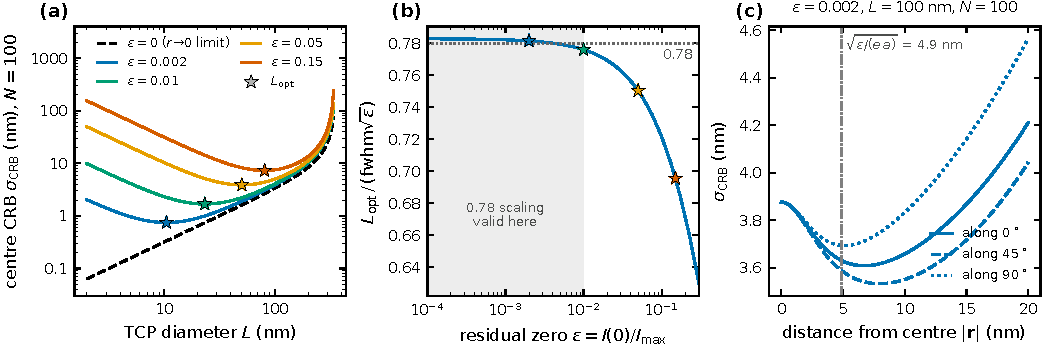
\includegraphics[width=\textwidth]{figures/fig7_zero_depth.pdf}
\caption{Finite zero depth ($\fwhm=\pnum{fwhm_nm}\src{fwhm_nm}$\,nm, $N=100$, Gaussian pedestal).
(a)~Centre CRB versus $L$ for $\epsilon=0.002$, $0.01$, $0.05$, $0.15$ (stars: $L_{\mathrm{opt}}$)
and for $\epsilon=0$ ($r\to0$ limit), which has no optimum and diverges at the ring diameter.
(b)~$L_{\mathrm{opt}}/(\fwhm\sqrt\epsilon)$ versus $\epsilon$: the value
\pnum{L_opt_over_fwhm_sqrt_eps_eps0p002}\src{L_opt_over_fwhm_sqrt_eps_eps0p002} at
$\epsilon=0.002$ holds only for $\epsilon\lesssim0.01$ (shaded) and falls to
\pnum{L_opt_over_fwhm_sqrt_eps_eps0p15}\src{L_opt_over_fwhm_sqrt_eps_eps0p15} at $\epsilon=0.15$.
(c)~CRB (nm) versus distance from the centre along three directions for $\epsilon=0.002$,
$L=100$\,nm: the minimum lies off the centre; the dash-dotted line marks the transition scale
$\sqrt{\epsilon/(ea)}=\pnum{zero_depth_transition_scale_nm}\src{zero_depth_transition_scale_nm}$\,nm,
a scale and not the position of the minimum.}
\label{fig:zerodepth}
\end{figure*}

\begin{figure*}[t]
\centering
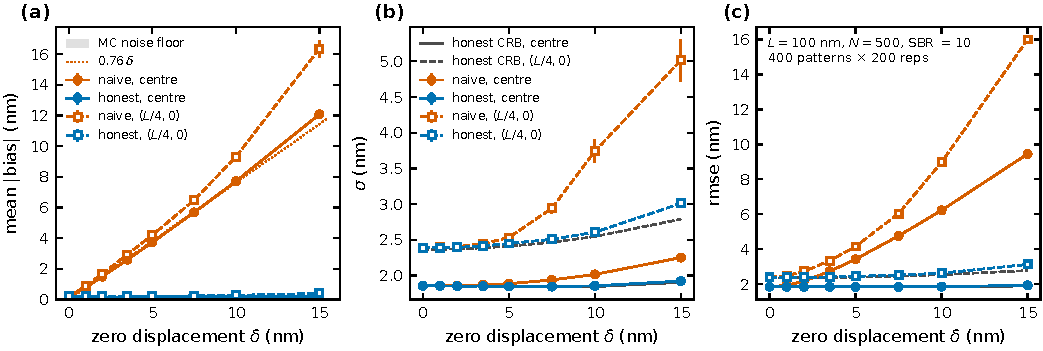
\includegraphics[width=\textwidth]{figures/fig8_misalignment.pdf}
\caption{TCP misalignment, i.e.\ an error in the positions of the zeros with the donut shape
unchanged ($L=100$\,nm, $N=500$, $\sbr=10$; all four zeros displaced by $\delta$
in random directions; $400$ patterns $\times$ $200$ repetitions; error bars are between-pattern
SE). (a)~Mean $|\text{bias}|$ of the naive MLE (nominal pattern) and of the honest MLE (true
pattern) versus $\delta$, at the centre and at $(L/4,0)$, with the MC noise floor (grey band) and
a straight line fitted to the naive centre points over all seven $\delta$ values including
$\delta=15$\,nm (dotted). The main slope estimate is the noise-free population value,
\pnum{misalignment_naive_bias_over_delta_pop_center}\src{misalignment_naive_bias_over_delta_pop_center}
at the centre and
\pnum{misalignment_naive_bias_over_delta_pop_Lq}\src{misalignment_naive_bias_over_delta_pop_Lq}
at $(L/4,0)$, growing with $\delta$. (b)~$\sigma$ and (c)~rmse versus $\delta$, with the CRB of
the true pattern: at the centre the naive $\sigma$ changes little and its loss is bias, whereas
at $(L/4,0)$ the naive $\sigma$ also grows, from
\pnum{misalignment_naive_sigma_Lq_d0_nm}\src{misalignment_naive_sigma_Lq_d0_nm} to
\pnum{misalignment_naive_sigma_Lq_d10_nm}\src{misalignment_naive_sigma_Lq_d10_nm}\,nm at
$\delta=10$\,nm; the honest $\sigma$ follows the CRB at
the centre and lies slightly above it at $(L/4,0)$.}
\label{fig:misalignment}
\end{figure*}
